\subsection{Consensus Ordering}
In the Tagion implementation of the Hashgraph algorithm, an Event is only allowed to point to one or none ``other parent'' which is called a ``father-event'' as shown om \cref{fig:consensus_order}. This strategy aids in solving the graph forking problem and simplifies the consensus ordering.\\
The ``self-parent'' is defined as a ``mother-event'' in the Tagion implementation. An event must have a mother-event but doesn't have to have a father-event.

Each event points to the previous event called the mother-event, and some also point to another father-event. The mother-event is defined as the previous event from the same node. The father is an event sent via the gossip network from another node. \\

The order $\Omega$ is calculated as:

%\end{equation}
\begin{equation}
 \Omega_{B,k+1} = max \big(\Omega_{A,k} , \Omega_{B,k} \big) +1
\end{equation}

The events in the epoch list are sorted by the order $\Omega$. If the order of two events is equal, the hash $h$ of the event is used to calculate the order.
The following expression is used to order the events:

\begin{align}
 {l}(A,B) & = 
    \begin{cases}
         {l'}(A,B) &  	\text{if}  ~ ({\Omega}_{A} = {\Omega}_{B} )  \\ 
        {{\Omega}_{A} < {\Omega}_{B}} & 
        \text{otherwise}
    \end{cases} 
    \label{equ:order}    
\end{align}

\begin{align}
{l'}(A,B) & = 
\begin{cases}
{l}(A_{mother},B_{mother}) &  	
\text{if}  ~ (\text{A has a mother} ~ \&  ~ \text{B has a mother}) \\ 
{l}(A_{father},B_{father}) &  	
\text{if}  ~ (\text{A has a father} ~ \&  ~ \text{B has a father}) \\ 
0 &  	
\text{if}  ~ (\text{A has a no father}) \\ 
1 &  	
\text{if}  ~ (\text{B has a father}) \\ 
H (    {h}_{A} \parallel {h}_{B} )  < H (    {h}_{B} \parallel {h}_{A} ) & 
\text{otherwise}
\end{cases} 
\end{align}



If parameter $l(A,B)$ is $'true'$ if event A is ordered before event B (see \cref{sec:)

\begin{figure}[H]
 \centering
 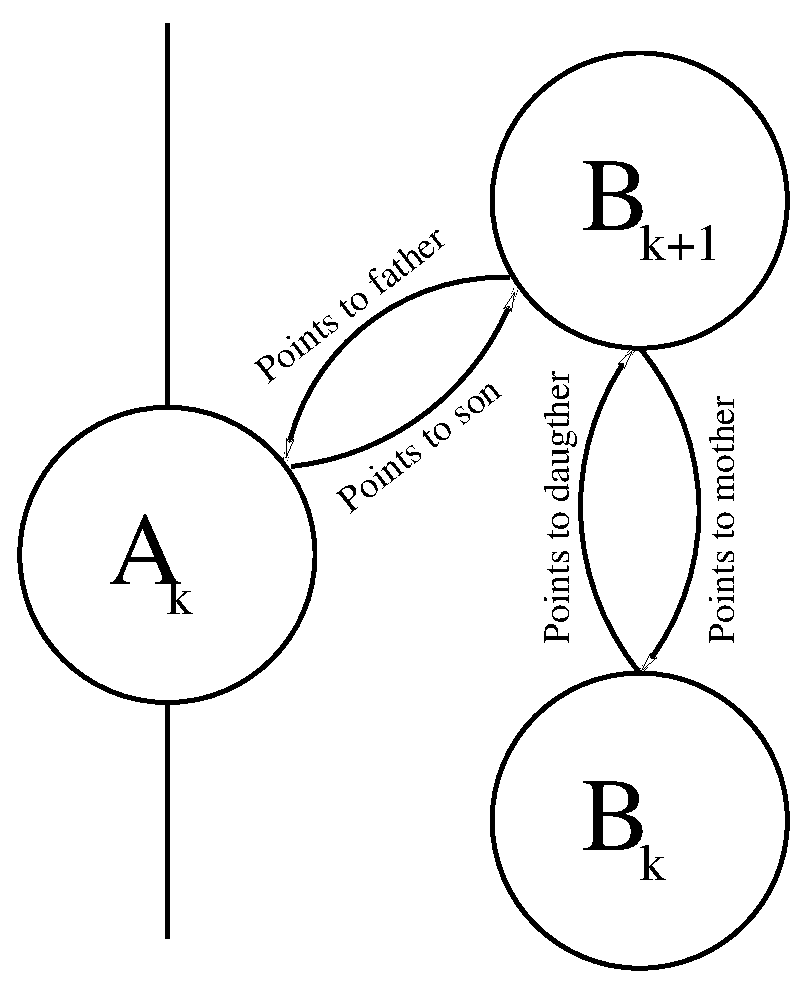
\includegraphics[width=0.5\textwidth]{fig/consensus_order.eps}
 % consensus_order.eps: 1550x1908 px, 300dpi, 13.12x16.15 cm, bb=0 0 372 458
 \caption{Events and relations}
 \label{fig:consensus_order}
\end{figure}
